%Man, robots are hard.... But the only book you'll need is
%\cite{Gibson79}. \note{Is self-citing tacky?}

%%%%%%%%%%% First paragraph - Motivating time to collision %%%%%%%%%%%%%
Automated collision avoidance technology is an indispensable part of mobile robots. As an alternative to traditional approaches using multi-modal sensors, purely image based collision avoidance strategies \cite{gandhi}, \cite{DroNet} have recently gained attention in robotics. These image-based approaches use the power of large data to detect immediate collision as a binary variable - collision or no collision. In this work, we propose a more fine-grained approach to predict the exact time to near-collision from images, with a much longer prediction horizon.  

   \begin{figure}[t]
      \centering
      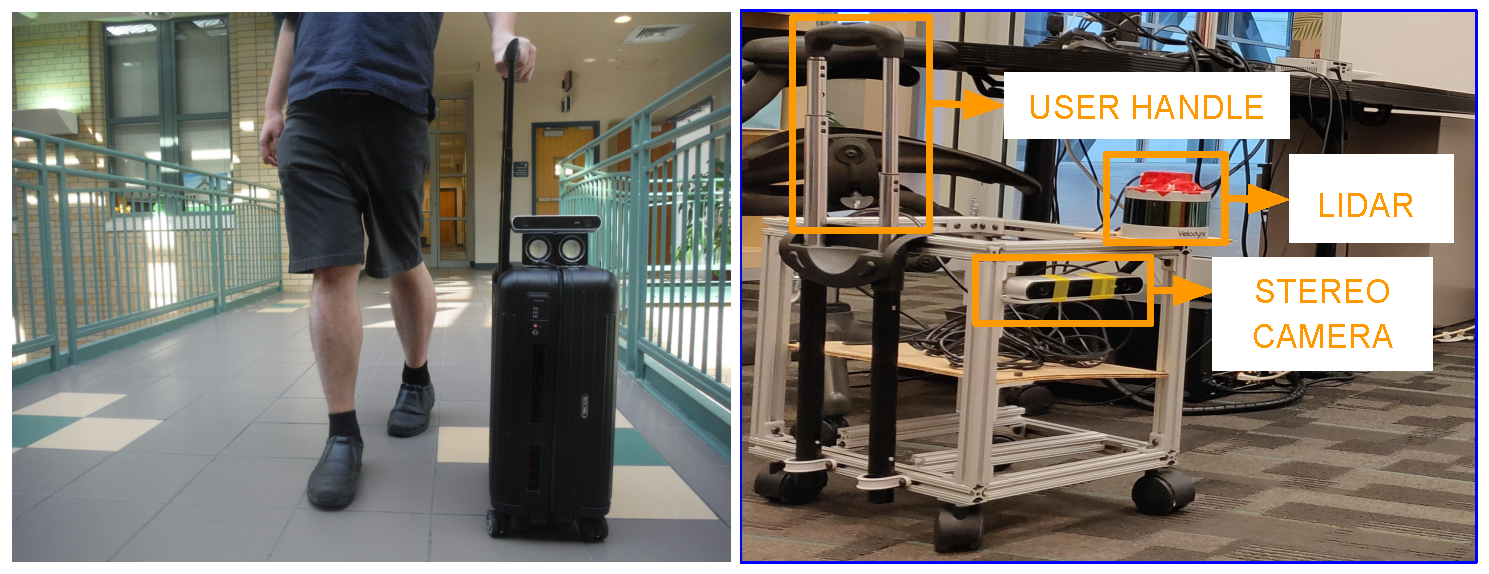
\includegraphics[height=5.5cm, width=\columnwidth]{figs/aspect_ratio_setup.pdf}
      \caption{The left image shows an assistive suitcase with a camera sensor and speaker to guide people. The right image shows the corresponding suitcase-shaped training prototype mounted with stereo camera and LIDAR for data collection.}
      \label{fig:setup}
   \end{figure}

%%%%%%%%%% Second paragraph - Anticipating common arguments %%%%%%%%%%%%%%%%%%%
A method frequently used for forecasting time to near-collision is to track the 3D location of the surrounding pedestrians and extrapolate their trajectories using a constant velocity model \cite{SIPP}, \cite{BBeep}. When it is possible to use high quality depth imaging devices, this type of physics-based modeling can be very accurate. However, physics-based approach can also be prone to failure in the presence of sensor noise and uncertainty in detection of nearby pedestrians. Small mistakes in the estimation of depth (common to low-cost depth sensors) or noise in 2D bounding box detection (common to image-based object detection algorithms) can be misinterpreted to be very large changes of velocity. Many physics-based approaches can be brittle in the presence of such noise. Accordingly, errors in either pedestrian detection, tracking or data association can result in very bad future trajectory estimates. Other more advanced physics-based models and decision-theoretic models also depend heavily on accurate state estimates of nearby people and can be significantly influenced by sensor and perception algorithm noise. We propose to address the issue of sensor noise and perception algorithm noise by directly estimating the time to near-collision from a sequence of images.
   
%%%%%%%%% Fourth paragraph - How did we go about creating the dataset? %%%%%%%%%%%%%%%%%%%%%%%%   
To create a dataset for learning time to collision, we designed a training prototype as shown in Fig. \ref{fig:setup}. It is both unnatural and infeasible to record or insist that people actually collide with the mobile platform to collect large scale data. As an abstraction, we define the presence of a person within a 1 meter radius around the mobile platform as a near-collision. If a person other than the user is present within this radius, we mark it as a near-collision that should be forecasted using an earlier segment of video. The proposed approach is designed for a mobile robot that is being pushed by a person with visual impairment as shown in Fig. \ref{fig:setup}. The goal of the system is to forecast the time to near collision, at most 6 seconds before the near collision event. While most of the existing datasets for human trajectory prediction are from a fixed overhead camera \cite{2009YoullNW}, \cite{UCY}, our dataset of \textbf{13,658} video segments targets the first-person view which is more intuitive for mobile robots. In the work on robust multi-person tracking from mobile platforms \cite{Andreas}, the dataset is egocentric at walking speed but with 4788 images it is insufficient to deploy the success of convolutional neural networks. 


%%%%%%%%% Fifth paragraph - Technical part, how exactly we are learning %%%%%%%%%%%%%%%
We formulate the forecasting of time to near-collision as a regression task. To learn the mapping from spatial-temporal motion of the nearby pedestrians to time to near-collision, we learn a deep network which, takes a sequence of consecutive frames as input and outputs the time to near-collision. To this end, we evaluate and compare two popular video network architectures in the literature: (1) The high performance of the image-based network architectures makes it appealing to reuse them with as minimal modification as possible. Thus, we extract the features independently from each frame using an image-based network architecture (\emph{e.g.}, VGG-16) and then aggregate the features across the temporal channels; (2) It is also natural to directly use a 3D ConvNet (\emph{e.g.}, I3D \cite{i3d}) to learn the seamless spatial-temporal features.

Moreover, it is a nontrivial task to decide how many past frames should form the input. Thus, we do extensive experimentation on different temporal windows as input using aforementioned video network architectures. Our results show that our proposed multi-stream CNN trained on the collected dataset is the best model for predicting time to near-collision.


In summary, the contributions of our work are as follows: (1) We contribute a large-scale dataset of \textbf{13,658} egocentric video snippets of humans navigating in indoor hallways. In order to obtain ground truth annotations of human pose, the videos are provided with the corresponding 3D point cloud from LIDAR; (2) We explore the possibility of forecasting the time to near-collision directly from a single RGB camera; (3) We provide an extensive analysis on how current state-of-the-art video architectures perform on the task of predicting time to near-collision on the proposed dataset and how their performance varies with different temporal windows as input.